%\documentclass[a4paper, 12pt, BCOR5mm, footsepline, parskip+, chapterprefix, smallheadings, footexclude, headexclude, DIV14, abstracton, pointlessnumbers, tablecaptionabove]{scrreprt}
\documentclass[
  parskip=half,
  paper=a4, 12pt, BCOR5mm, DIV14,
  footsepline, chapterprefix,
  abstract=true,
  headings=small,
  footinclude=false,
  headinclude=false,
  numbers=noenddot,
  captions=tableheading,
  listof=totoc
]{scrreprt}

%===========================================================
% page layout
%\usepackage[activate=normal]{pdfcprot}
\usepackage{scrpage2}
\pagestyle{scrheadings}
% ARTICLE: remove the following two lines if you are in article mode
\renewcommand*{\chapterpagestyle}{scrheadings}
\renewcommand*{\partpagestyle}{empty}
\renewcommand{\headfont}{\normalfont\sffamily\bfseries}
\renewcommand{\pnumfont}{\normalfont\sffamily\bfseries}
\newcommand{\seeSec}[1]{see Section \ref{#1}}
\newcommand{\seeFig}[1]{see Figure \ref{#1}}
\automark{chapter}
\cfoot{}
\chead{}
%\lefoot{\pagemark}
\ofoot{\headmark \hspace{1em} \hspace{1em}\pagemark}
\ohead{}
%===========================================================

\usepackage[T1]{fontenc}
\usepackage[utf8x]{inputenc}
\usepackage[english]{babel}
\usepackage{lmodern}

\usepackage{makeidx}
\makeindex

%\usepackage{enumerate}
\usepackage{enumitem}
\usepackage{xparse}
\DeclareDocumentCommand\itembf{mg}{%
  {\item{\sffamily{\bfseries #1}\IfNoValueF{#2}{ (#2)}.}\enspace}%
}
\newcommand{\boldul}[1]{\textbf{\underline{#1}}}

\usepackage[colorlinks,linkcolor=blue]{hyperref}
\usepackage[all]{hypcap} % link to top of images
\usepackage[acronym,toc,nomain,nonumberlist,section=chapter]{glossaries}
\makeglossary

\usepackage[tikz]{bclogo}

% ------------------------------------------------------------------------------

\author{}
\title{C-130J Super Hercules \\
\large Flight Manual}

% ------------------------------------------------------------------------------
\begin{document}

\selectlanguage{english}

\maketitle

\sffamily
{
Copyright \copyright~2013 by Thomas Geymayer\\
Some Rights Reserved. "C-130J Super Hercules - Flight Manual" is licensed under a Creative Commons Attribution-Noncommercial-Share Alike 3.0 Unported License.

\subsection*{You are free:}

\textbf{To Share} -- to copy, distribute, display, and perform the work\\
\textbf{To Remix} -- to make derivative works

\subsection*{Under the following conditions:}

\textbf{Attribution} -- You must attribute the work in the manner specified by the author or licensor (but not in any way that suggests that they endorse you or your use of the work). (Visibly include the title and author's name in any excerpts of this work.)

\textbf{Noncommercial} -- You may not use this work for commercial purposes.

\textbf{Share Alike} -- If you alter, transform, or build upon this work, you may distribute the resulting work only under the same or similar license to this one.

\subsection*{With the understanding that:}

\textbf{Waiver} -- Any of the above conditions can be \boldul{waived} if you get permission from the copyright holder.

\textbf{Public Domain} -- Where the work or any of its elements is in the \boldul{public domain} under applicable law, that status is in no way affected by the license.

\textbf{Other Rights} -- In no way are any of the following rights affected by the license:
\begin{itemize}
  \item Your fair dealing or \boldul{fair use} rights, or other applicable copyright exceptions and limitations;
  \item The author's \boldul{moral} rights;
  \item Rights other persons may have either in the work itself or in how the work is used, such as \boldul{publicity} or privacy rights.
\end{itemize}

This is a human-readable summary of the \boldul{Legal Code (the full license)}, located here:\\
\url{http://creativecommons.org/licenses/by-nc-sa/3.0/legalcode}
}


\tableofcontents

\chapter{Introduction}

\begin{bclogo}[logo=\bcattention, ombre=false, couleurBarre=red, marge=18, noborder=true]{ Warning}
An operating procedure, technique, etc., that may result in personal injury or loss of life if not carefully followed.
\end{bclogo}

\begin{bclogo}[logo=\bctakecare, ombre=false, couleurBarre=orange, marge=18, noborder=true]{ Caution}
An operating procedure, technique, etc., that may result in damage to equipment if not carefully followed.
\end{bclogo}

\begin{bclogo}[logo=\bclampe, ombre=false, couleurBarre=blue, marge=18, noborder=true]{ Note}
An operating procedure, technique, etc., that is considered essential to emphasize.
\end{bclogo}

\newacronym{EGT}{EGT}{Exhaust Gas Temperature}

%\newcommand{\newrefgloss}[3]{\newglossaryentry{#1}{name=#1,text={\hyperref[#3]{#1}},description={\hyperref[#3]{#2}}}}
\newcommand{\newrefgloss}[3]{\newglossaryentry{#1}{name=#1,text={#1},description={\hyperref[#3]{#2}}}}
\newcommand{\newgloss}[2]{\newglossaryentry{#1}{name=#1,description=#2}}
\newcommand{\newacro}[2]{\newacronym{#1}{#1}{#2}}

\newrefgloss{ACAWS}{Advisory, Caution and Warning System}{sec:acaws}
\newrefgloss{AMU}{Avionics Management Unit}{sec:amu}
\newrefgloss{APU}{Auxiliary Power Unit}{sec:apu}
\newacro{A/T}{Auto Throttle}

\newacro{BIU}{Bus Interface Unit}

\newacro{CADC}{Central Air Data Computer}
\newacro{CAPS}{Coordinated Aircraft Positioning System}
\newglossaryentry{CAPS-airdrop}{name=CAPS,text=CAPS,description={\hyperref[sec:caps-airdrop]{Combat Airdrop Planning System}}}
\newacro{CAWS}{Caution, Advisory and Warning System}
\newacro{CDI}{Course Deviation Indicator}
\newacro{CMDS}{Counter Measures Dispensing System}
\newacro{CMDU}{Color Multipurpose Display Unit}
\newacro{CNBP}{Communication/Navigation/Breaker Panel}

\newrefgloss{ECHS}{Enhanced Cargo Handling System}{sec:echs}

\newacro{FPA}{Flight Path Angle}

\newrefgloss{HDD}{Head Down Display}{chap:hdd}
\newrefgloss{HSI}{Horizontal Situation Indicator}{sec:hsi}

\newacro{IAS}{indicated airspeed}

\newgloss{kVA}{kilo Volt-Ampere}

\newgloss{lbs/hr}{pounds per hour}

\newrefgloss{MFCD}{Multi Functional Control Display}{sec:mfcd}

\newacro{OSB}{Option Select Button}

\newrefgloss{PFD}{Primary Flight Display}{sec:pfd}
\newgloss{psi}{pressure in pounds per square inch}

\newrefgloss{RECP}{Ramp and Emergency Control Panel}{sec:recp}
\newgloss{RPM}{Revolutions Per Minute}


\part{The Aircraft}
\chapter{General Description}

\chapter{Systems}

\section{Auxiliary Power Unit (APU)}
\label{sec:apu}

A Honeywell Aerospace GTCP85-180L \gls{APU} is located in the forward part of the left wheel well. The \gls{APU} is a small, self-contained, single shaft gas turbine operating at a constant speed of approximately 42.000 \gls{RPM}. A shaft driven 40 \gls{kVA} AC generator supplies power to the electrical system. During ground operation bleed air can be used for engine starting and operation of the air-conditioning systems. Using the aircraft battery to start the \gls{APU} allows for operations on remote locations, without any ground support equipment available.

%Electrical starter, control circuits and ignition are powered through the Isolated DC bus.

\subsection{Fuel System}

The APU uses the same fuel as used for the main engines. Depending on the applied load, typical fuel consumption varies between 130 \gls{lbs/hr} and 270 \gls{lbs/hr}.

\paragraph*{Fuel Supply}
Fuel is gravity feed from the No. 2 main tank through a firewall shutoff valve installed in the No. 2 dry bay. The shutoff valve prevents fuel flow anytime the \gls{APU} control switch is placed in the STOP position, the \gls{APU} fire handle is pulled or the \gls{APU} control circuits are deengerized.

\paragraph*{Fuel Control Unit}
The fuel control unit fully automatically operates the fuel pump. Using a shaft governor the amount of fuel supplied to the combustor is varied to keep the rotational speed constant. A thermostat limits the fuel flow to protect the turbine from overtemperature, effectively also limiting acceleration during starting. While extracting bleed air, temperature limiting is shifted to the \nameref{par:bleed-air-shutoff-and-load-control-valve}.

\paragraph*{Fuel Shutoff Valve}
\label{par:fuel-shutoff-valve}
At the outlet of the fuel control unit another fuel shutoff valve opens once reaching a minimum oil pressure. During startup it opens at approximately 10\% \gls{RPM}. If oil pressure is lost the valve closes and the \gls{APU} will automatically shut down.

\subsection{Oil System}

A pressurized oil system provides lubrication to gears and shaft bearings. The shaft driven oil pump delivers oil from an external reservoir to the gears and bearings. A relieve valve maintains an operating pressure within 90$\pm$10 \gls{psi} while the \gls{APU} operates at 100\% \gls{RPM}. Oil temperature is regulated by either directing oil flow through the oil cooler, or if oil temperature is below 27°C, through the oil cooler by-pass valve.

\paragraph*{Oil-pressure sequencing switch}
At approximately 15\% \gls{RPM} oil pressure is sufficient to operate the oil-pressure sequencing switch, which completes circuits to the \nameref{par:fuel-shutoff-valve} and ignition system. It prevents starting without lubrication and ensures an adequate airflow for combustion before introducing fuel and initiating ignition.

\paragraph*{Door-control oil-pressure switch}
Oil pressure below 20 \gls{psi} (equals approximately 18\% \gls{RPM}) operates the door-control oil-pressure switch allowing to close the \nameref{par:air-intake-door}. This is done to prevent collapse of the air inlet duct due to build-up of negative pressure.

%\begin{bclogo}[logo=\bclampe, ombre=true, couleurOmbre = black!80, couleurBarre=blue, marge=6]{Note}
\begin{bclogo}[logo=\bclampe, ombre=false, couleurBarre=blue, marge=18, noborder=true]{Note}
\indent
Placing the APU control switch in the "STOP" position or pulling the APU fire handle is required to complete the circuit for actually closing the \nameref{par:air-intake-door}.
\end{bclogo}

\subsection{Airflow}

\paragraph*{Air Intake Door}
\label{par:air-intake-door}

\paragraph*{Bleed Air Shutoff and Load Control Valve}
\label{par:bleed-air-shutoff-and-load-control-valve}

\subsection{Controls and Indications}

\nameref{sec:apu-panel} and \nameref{sec:bleed-air-panel}

%40 KVA AC generator, electrical power up to 20.000 feet.

%APU air inlet door closes if APU control switch is in STOP position and oilpressure decreases below approximately 20 PSI, which happens at about 18 percent \gls{RPM}.

%Starter approx. 1100 Watt. inrush current 4-8 times normal

APU bleed air valve switch on the Bleed Air Panel.

\section{Advisory, Caution and Warning System (ACAWS)}
\label{sec:acaws}

\gls{ACAWS}

\section{Electric System}

2 batteries: Utility, Avionics 24V 42Ah at C1

\#2 generator powers essential AC bus, if \#2 lost APU powers essential AC bus (APU always powers essential AC bus if online), else \#1 takes load (same side takes/assumes load). If two engines/generators on same side shutdown/lost, symmetrical engines pick up loads.

\#1 generator: Left Hand AC bus.\\
\#2 generator powers Essential AC bus.\\
\#3 generator will power the Main AC bus.\\
\#4 generator will power the Right Hand AC bus.

Gen 1-4 and APU ACAWS Indications. When the GCU detects an out of tolerance condition, and a generator switch or EXT PWR/OFF/APU switch is in ON (generator) or APU (apu), it will open the line contactor and send a system status indication to the bus interface unit BIU. The
BIU will then generate a data word to the mission computer that a failure has occurred in one of the engine generators or the APU generator. An advisory, caution, and warning system (ACAWS) text message (GEN 1,2,3, or 4 FAIL or APU GEN FAIL) will then be displayed for the first ten
seconds in reverse color (black letters on a night vision imaging system (NVIS) yellow background) followed by flashing master caution lights.

\section{Avionics System}

The \gls{BIU}s convert various signals and serve as additional backup bus controllers (and somehow the Mission Computers?).

\section{Hydraulic System}

Utility hydraulic system: wing flaps, main landing gear, normal braking, nose wheel steering.

\section{Enhanced Cargo Handling System (ECHS)}
\label{sec:echs}

\gls{MFCD}, \gls{RECP}, \gls{CAWS} 12 pairs of electric pallet locks (40 inch spacing) http://www.google.com/patents/EP0771726A2?cl=en

\subsection{Cargo Compartements}

\begin{itemize}
  \itembf{C} 245 - 281
  \itembf{D} 281 - 337
  \itembf{E} 337 - 401
  \itembf{F} 401 - 457
  \itembf{G} 457 - 517
  \itembf{H} 517 - 597
  \itembf{I} 597 - 627
  \itembf{J} 627 - 682
  \itembf{K} 682 - 737
  \itembf{L} 737 - 803 (Ramp)
  \itembf{M} 803 - 869 (Ramp)
\end{itemize}

\subsection{Locks}

\begin{enumerate}
  \item 302
  \item 342
  \item 382
  \item 422
  \item 462
  \item 502
  \item 542
  \item 582
  \item 622
  \item 662
  \item 682
  \item 803?
\end{enumerate}

% right 884px/885px
% left 80px/87px
% total 800px -> l: 112px, r: 912

\chapter{Cockpit Controls}

Blah blah

\section{Overhead Panel}

\subsection{Electrical Panel}

\begin{enumerate}
  \itembf{Battery (BTRY) switch} Connects battery bus to isolated DC bus.
\end{enumerate}

\subsection{Bleed Air Panel}
\label{sec:bleed-air-panel}

\begin{enumerate}
  \itembf{\gls{APU} Bleed Air Valve switch}{OPEN/CLSD}
  \itembf{Divider Valve switch}{CLOSE/AUTO/OPEN}
  \itembf{Wing Isolation Valve switches}{CLOSE/AUTO/OPEN}
  \itembf{Nacelle Shutoff Valve switches}{CLOSE/AUTO/OPEN}
\end{enumerate}

\subsection{Fuel Management Panel}

Transfer switches (TO/FROM)

\subsection{Engine Start and Fire Control Panel}
\label{sec:eng-panel}

\begin{enumerate}
  \itembf{Engine 1/2/3/4 Fire Handle}
  \itembf{Engine 1/2/3/4 Start switch}
    \begin{itemize}
      \itembf{MOTOR}
      \itembf{STOP}
      \itembf{RUN}
      \itembf{START}
    \end{itemize}
    Fuel pumps in respective tank operated in RUN/START and stopped in MOTOR/STOP
\end{enumerate}

\subsection{APU Panel}
\label{sec:apu-panel}

The \gls{APU}...

\begin{enumerate}
  \itembf{Control switch}
    \begin{itemize}
      \itembf{STOP} Same as 110\% overspeed switch. APU door closes if below 18\% (or oilpressure below 20 PSIG).
      \itembf{RUN} APU door opens.
      \itembf{START}{spring-loaded position} If APU door opened at least 15° starter engages
    \end{itemize}
  \itembf{\gls{EGT} indication}
  \itembf{\gls{RPM} indication}
  \itembf{Fire handle} The T-shaped fire handle
    \begin{enumerate}
      \item Control power interrupt
      \item Fuel shut-off valve closes
      \item Once the APU \gls{RPM} falls below approximately 18\% the APU air intake door is closed.
      \item Agent discharge switching available
    \end{enumerate}
\end{enumerate}

\section{Instrument Panel}

\subsection{Avionics Management Unit (AMU)}
\label{sec:amu}

The \gls{AMU}, \gls{CNBP}, \gls{CMDU}, \gls{CMDS}

\subsection{Head Down Displays (HDD)}
\label{sec:hdd}

Readouts are color coded. Information will be presented in white when in the normal operating range, yellow for information out of the normal range but not out of limits, and red for out of limit values.

\newpage
\subsubsection{Primary Flight Display (PFD)}
\label{sec:pfd}

The \gls{PFD}...

%\newpage
\subsubsection{Engine}

\newpage
\subsubsection{System Status}

The SYSTEM STATUS display consists of multiple sections:

\begin{figure}[h]
  \centering
  \colorbox{black}{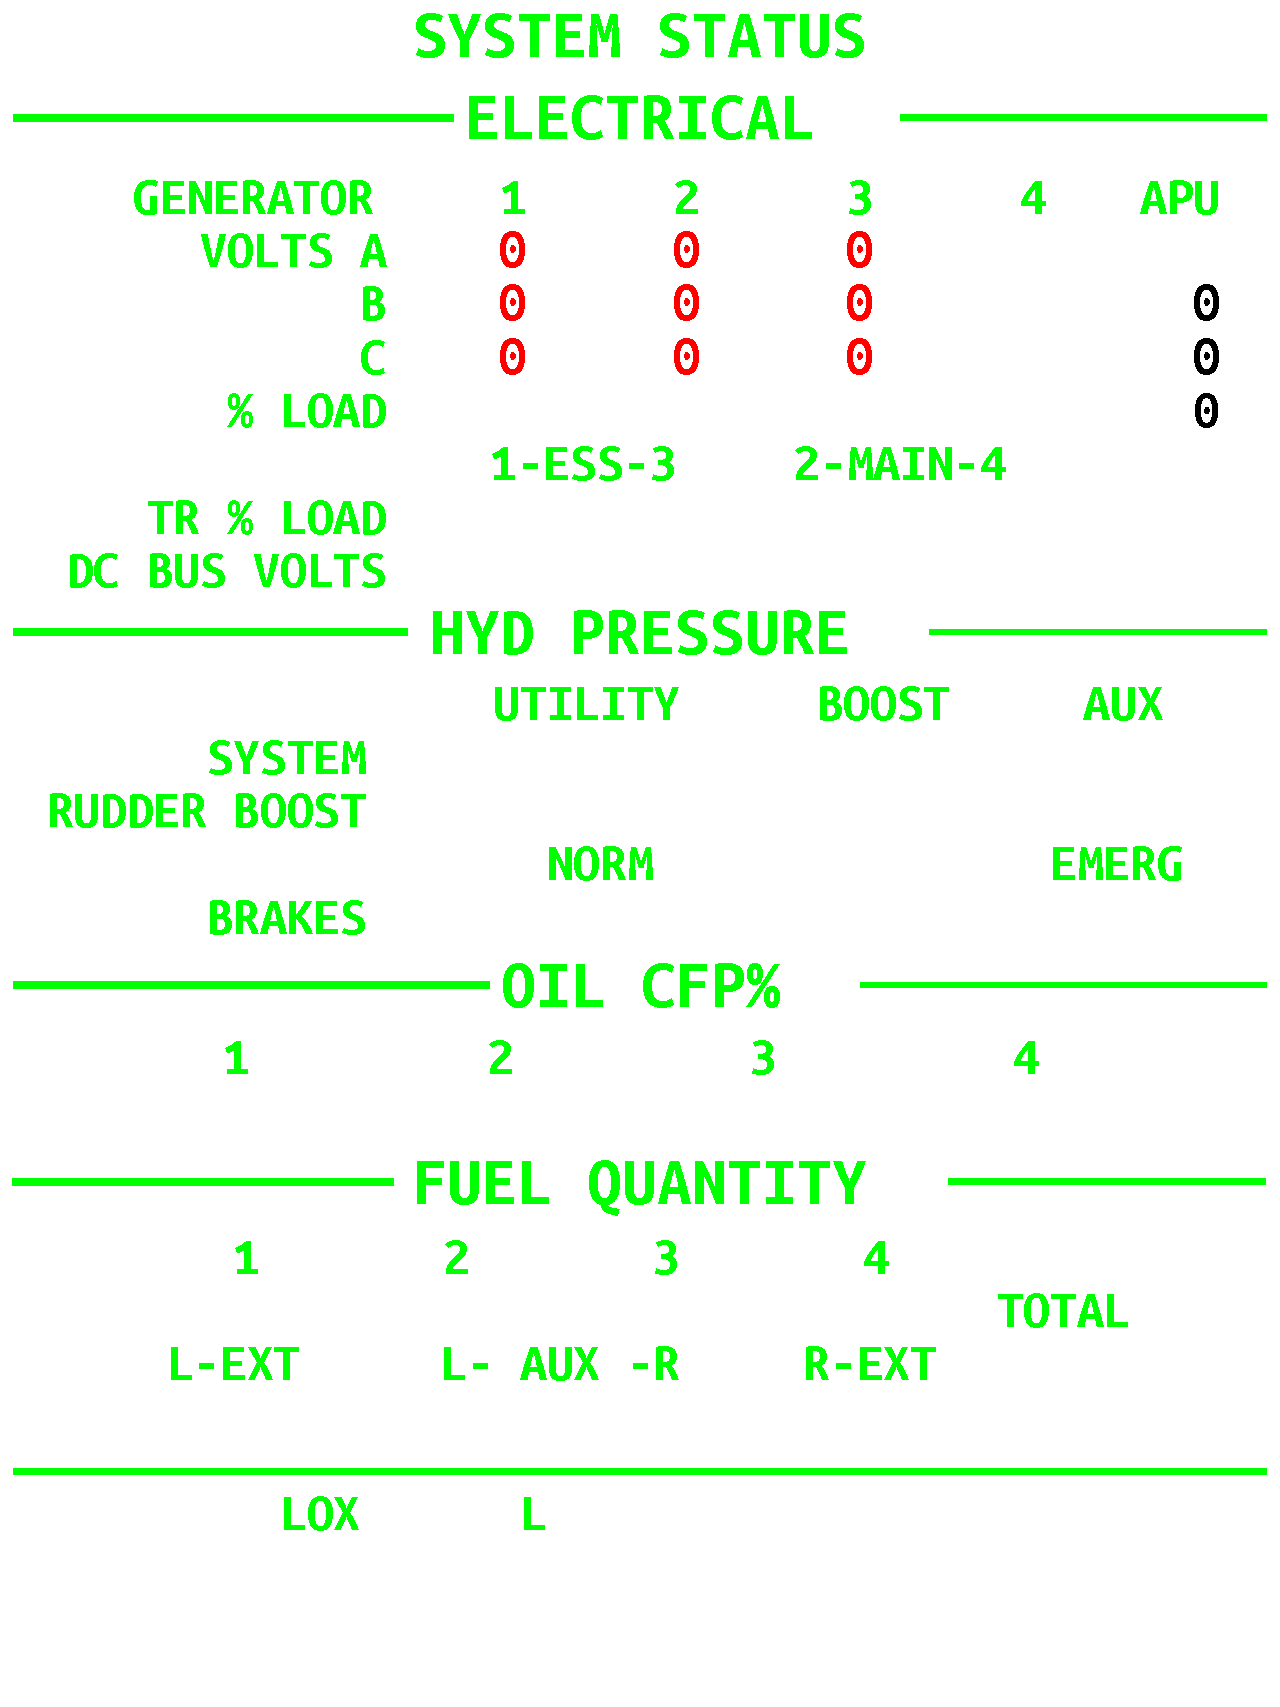
\includegraphics[width=7cm]{figures/hdd/SYSTEM-STATUS}}
  \caption{SYSTEM STATUS display}
\end{figure}

\paragraph*{ELECTRICAL}
Generator voltage and percentage of rated current load are shown. Values for generator voltage and load are displayed in columns, labeled from left to right, representing generators 1, 2, 3, 4 and the APU generator. Three voltages are shown in the column for each generator to indicate the voltage of each of the three phases of the generator: A phase, B phase, C phase. Percent of maximum rated load for all five generators (an average of the three phases) is displayed in the row below the C phase voltage. If the system is not powered, OFF will be displayed in the appropriate data blocks. If the system is disconnected (eg. EXT PWR/OFF/APU not APU for APU), three dashed lines will be displayed. The display symbols are generated by the multifunction display units based on information received from the mission computer. 

\paragraph*{HYD PRESSURE}

\paragraph*{OIL CFP\%}

\paragraph*{FUEL QUANTITY}

\subsection{Autopilot}

Reference Settings
\begin{enumerate}
  \itembf{HP}
  \itembf{RAD ALT} Radar altitude
  \itembf{IAS} \gls{IAS}
  \itembf{FPA} \gls{FPA}
  \itembf{MINS}
\end{enumerate}

Mode Selections
\begin{enumerate}
  \itembf{ALT}
  \itembf{VS} Vertical Speed
  \itembf{SEL}
  \itembf{IAS} \gls{IAS}
  \itembf{HDG} Heading
  \itembf{NAV}
  \itembf{CAPS} \gls{CAPS}
  \itembf{APPR}
  \itembf{A/T} \gls{A/T}
\end{enumerate}

REF SET\\
ALT SET\\
BARO SET

\section{Flight Controls}

\subsection{Yoke}

\paragraph*{Left side}
HUD DECLUTTER\\
?PH\\
RADIO\\
STOP WATCH

\paragraph*{Front/Right side}
ELEV TRIM (Dual Rocker Switch) NOSE DN / UP\\
?\\
SYN (VERT REF SET) (Pitch Synchronization)\\
?\\
G/A (GO AROUND)

\chapter{Cargo Compartement Controls}

\section{Loadmaster Station}

\subsection{Multi Functional Control Display (MFCD)}
\label{sec:mfcd}

\paragraph*{MENU}

Shows cargo compartment graphic and CAWS messages. Use Option Select Buttons (OSB) to change page. Use this page if \gls{ECHS} is not in use.

\paragraph*{ONLOAD/CURRENT CARGO?}

\paragraph*{OFFLOAD}

\paragraph*{COMBAT OFFLOAD}

\paragraph*{AIRDROP PROGRAM}

\paragraph*{AIRDROP}

\paragraph*{JETTISON}

\paragraph*{LOCK CONTROL}

\subsection{Ramp and Emergency Control Panel (RECP)}
\label{sec:recp}


\part{Electronic Flight Instruments}

% ==============================================================================
\chapter{Head Down Displays (HDD)}
\label{chap:hdd}

Readouts are color coded. Information will be presented in white when in the normal operating range, yellow for information out of the normal range but not out of limits, and red for out of limit values.

PFD Data Presentation: Coloring is used to further segregate differing sources of information. Cyan denotes Pilots input reference set, Amber denotes Flight director.

\newpage
\section{Primary Flight Display (PFD)}
\label{sec:pfd}

The \gls{PFD}, \gls{HSI}, ...

\begin{figure}[h]
  \centering
  \colorbox{black}{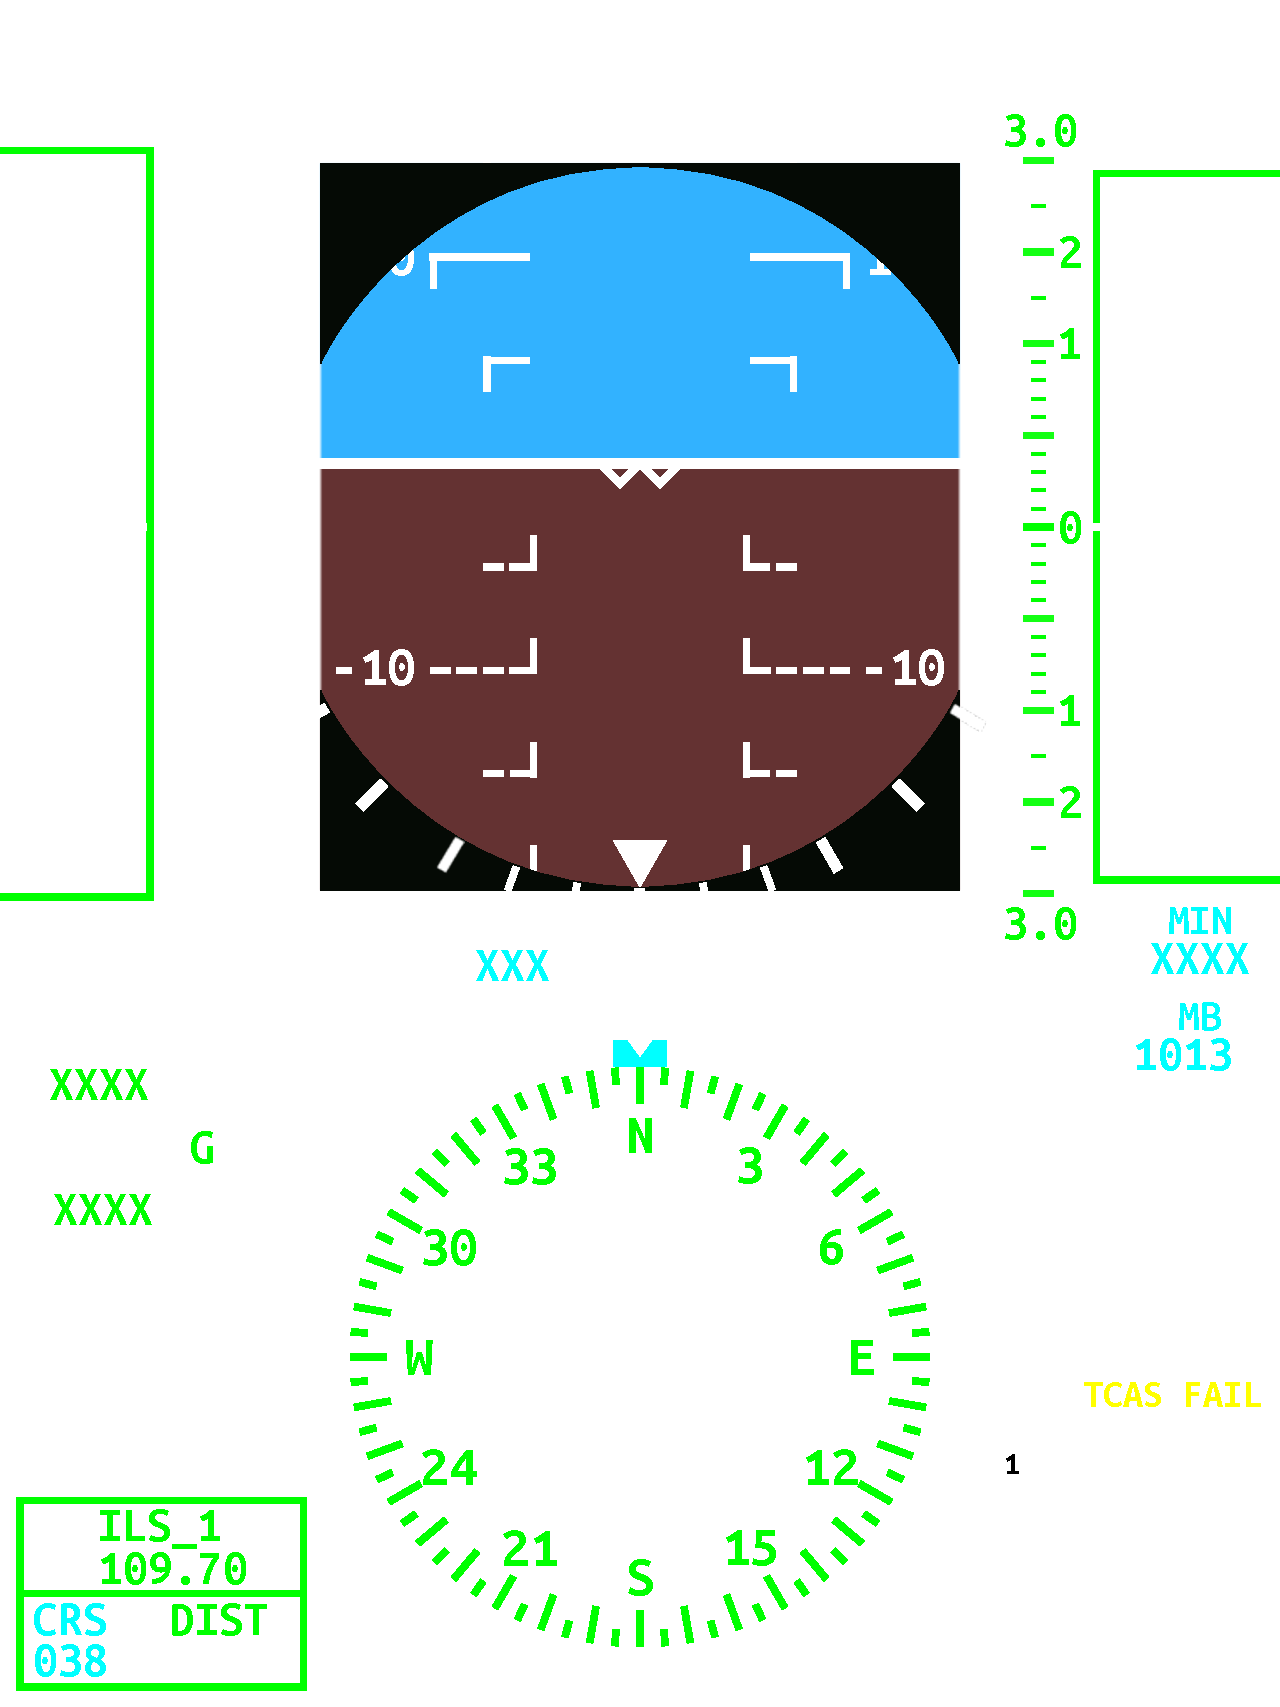
\includegraphics[width=7cm]{figures/hdd/PFD}}
  \caption{Primary Flight Display}
\end{figure}

cyan for VOR/ILS, magenta for FMS

Entered V1 and VR will automatically display on the airspeed indication.

\subsection{Horizontal Situation Indicator (HSI)}
\label{sec:hsi}

Displays Heading, Track, \gls{CDI}, Heading Bug (cyan), Bearing pointers (VOR green, ADF cyan)

\paragraph*{V Speeds}

\begin{itemize}
  \itembf{$V_1$} Critical engine failure recognition speed.
  \itembf{$V_R$} Rotation speed.
  \itembf{$V_{OBS}$} Obstacle clearance speed.
  \itembf{$V_{FUSS}$} Flaps Up Safety Speed.
  \itembf{$V_H$} Maximum speed in level flight at maximum continuous power. (recommended clean max. speed)
\end{itemize}

\paragraph*{Autopilot}

\begin{itemize}
  \item left-top (green): HDG, NAV CAPT, (BACK LOC)?
  \item left-bottom (white): NAV ARM

  \item right-top (green): ALT HOLD, GO ARND, GS CAPT, (CAT2)?
  \item right-bottom (white): ALT SEL, GS ARM, (CAT2 ARM)?
\end{itemize}

For coupled autopilot operation the altitude hold mode is automatically disengaged when:

\begin{itemize}
\item The elevator trim switch or pitch wheel is activated
\item When Vertical Speed (VS), pitch synchronization (SYN), or airspeed (IAS) mode is engaged
\item At glide slope capture in the APPR mode
\end{itemize}

At one thousand feet prior to the selected altitude (ascending or descending) a voice message of A THOUSAND TO GO will alert the crew to approaching altitude selection.

Inflight, the reference IAS cannot be set below 1.2 Vs. With weight on wheels, the reference airspeed is fixed to V2.

In the Primary Flight Display or Heads-Up Display, when either autopilot is engaged (pitch and roll axis), the shape of both Climb Dive Markers (CDM) change from a circle to a diamond.

\newpage
\section{Engine}

\begin{figure}[h]
  \centering
  \colorbox{black}{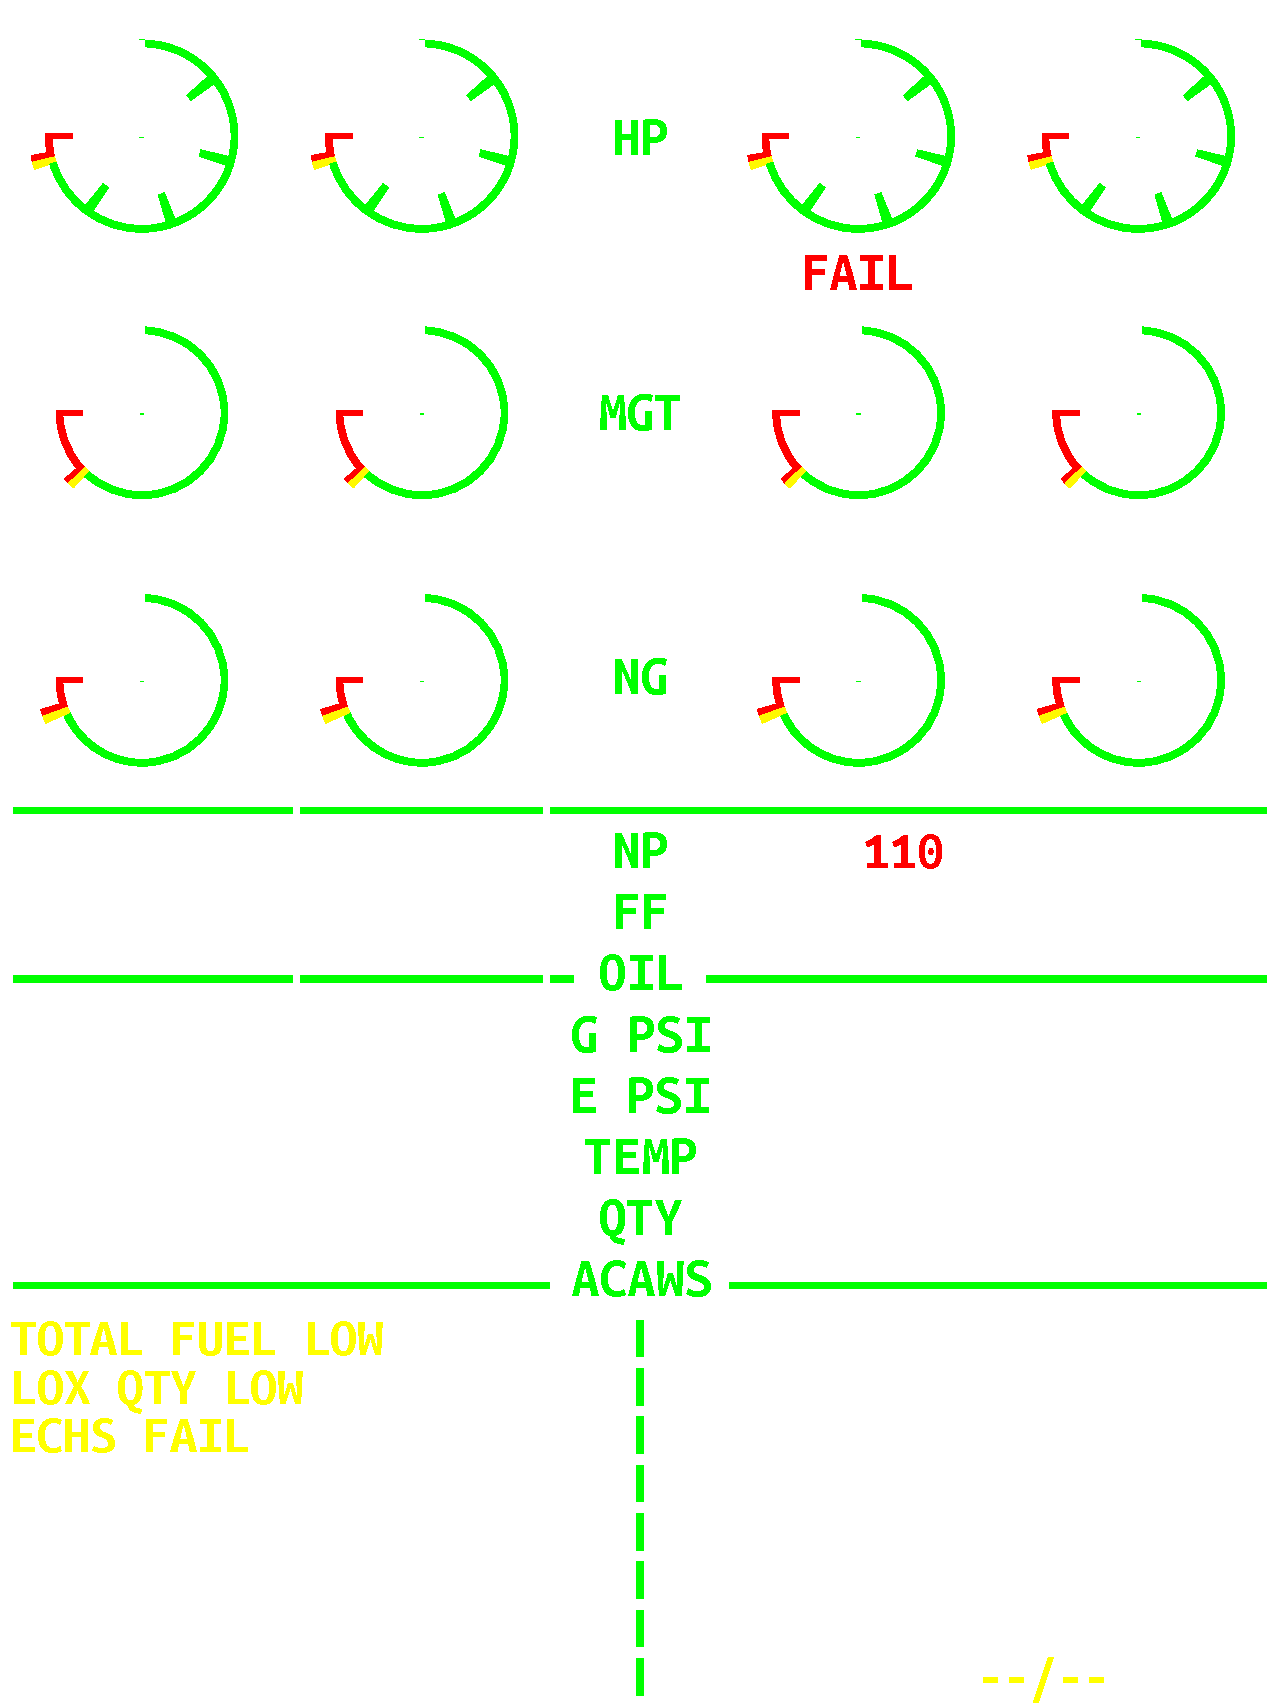
\includegraphics[width=7cm]{figures/hdd/EICAS}}
  \caption{ENGINE and ACAWS display}
\end{figure}

\newpage
\section{CAPS}
\label{sec:caps-airdrop}

\gls{CAPS-airdrop}

\begin{figure}[h]
  \centering
  \colorbox{black}{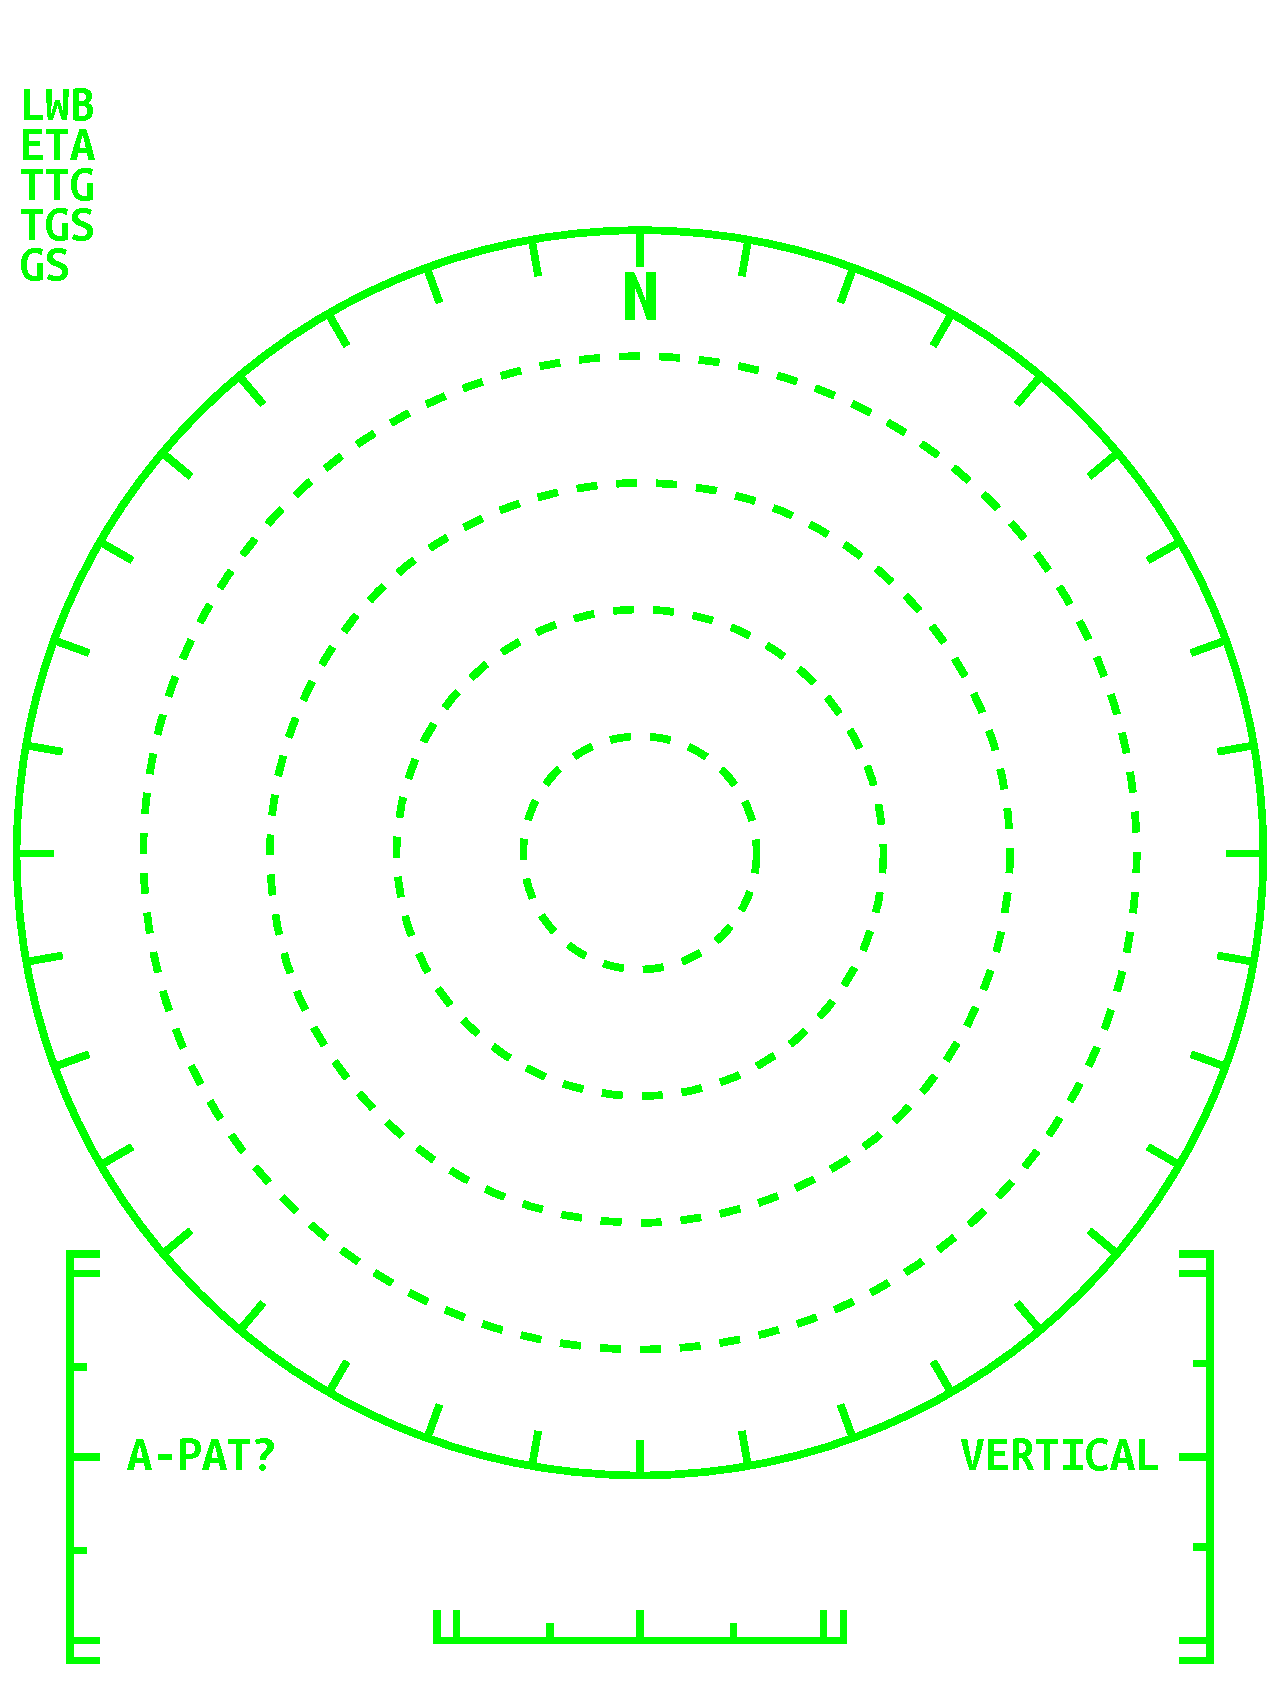
\includegraphics[width=7cm]{figures/hdd/CAPS}}
  \caption{\gls{CAPS-airdrop} display}
\end{figure}

\newpage
\section{System Status}

The SYSTEM STATUS display consists of multiple sections:

\begin{figure}[h]
  \centering
  \colorbox{black}{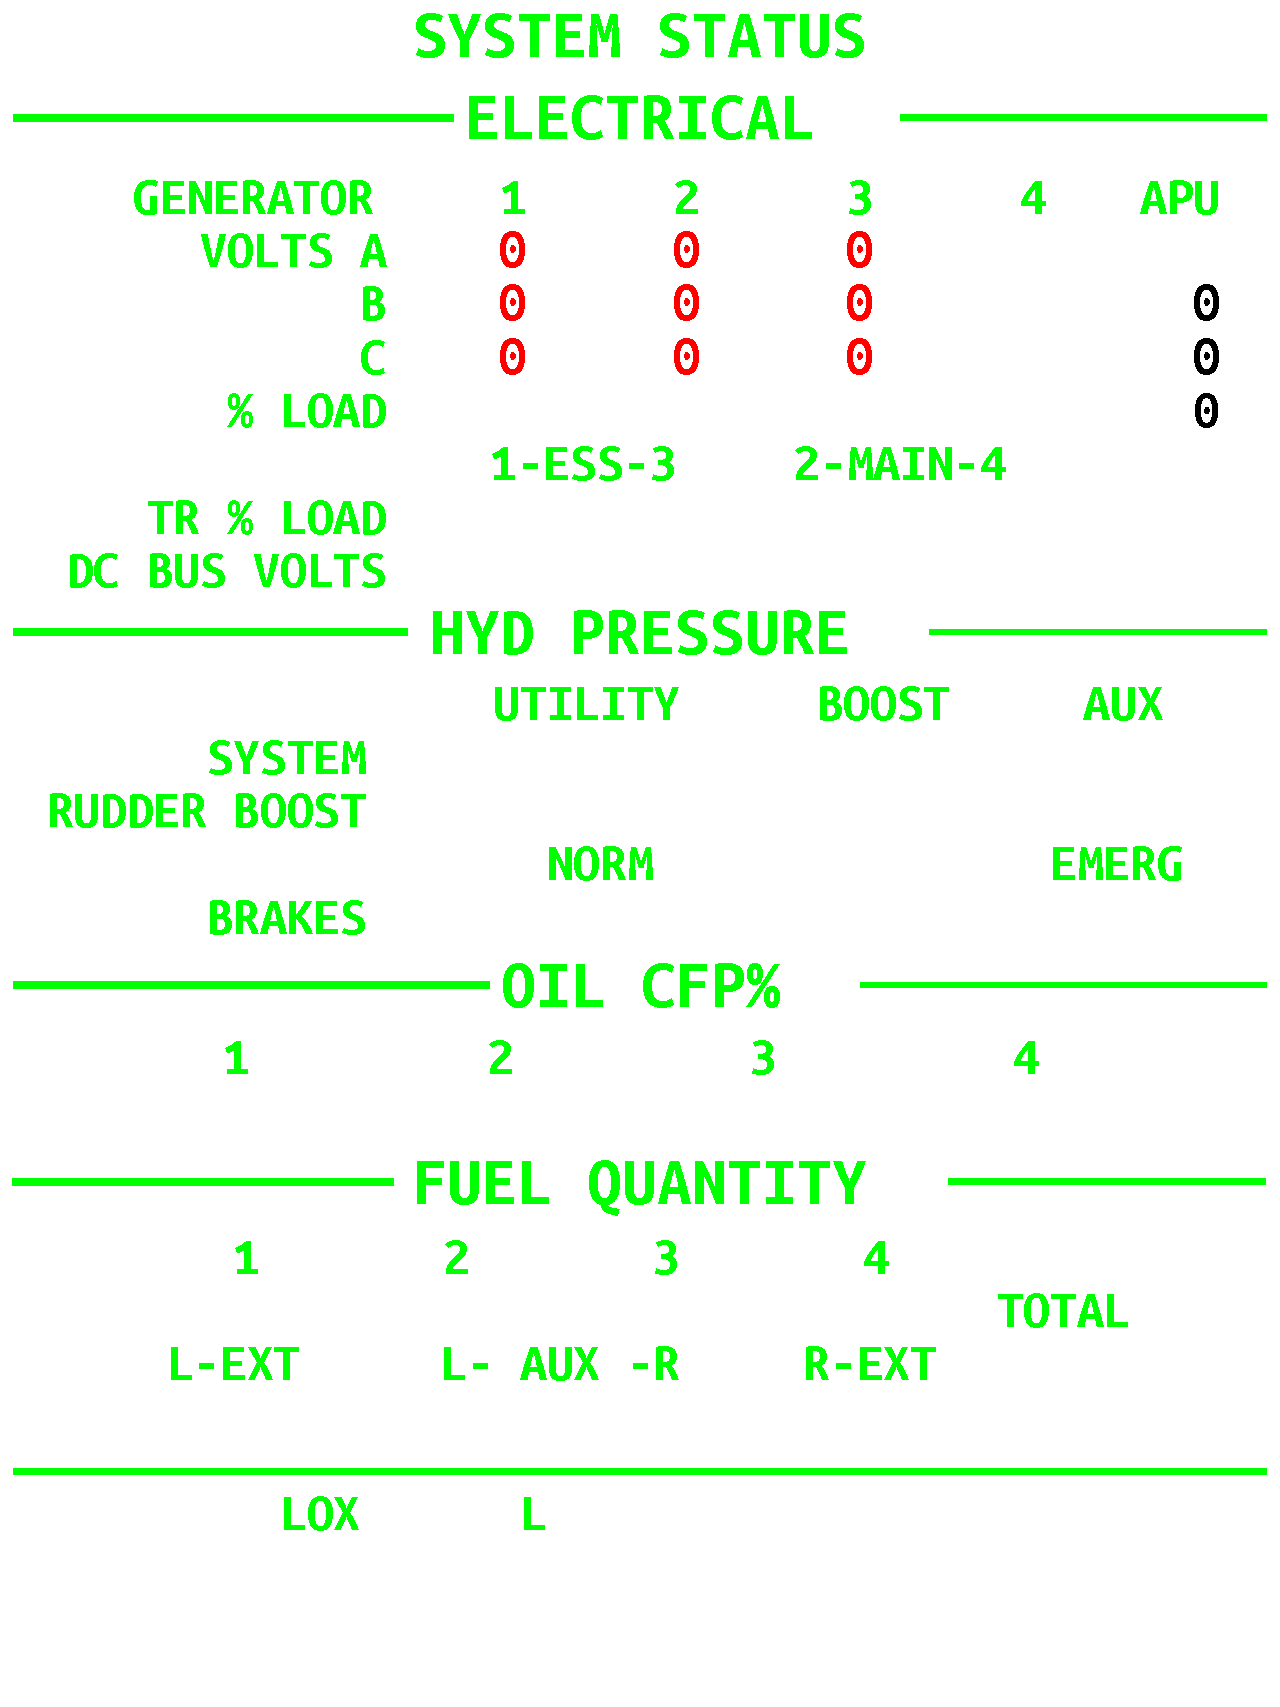
\includegraphics[width=7cm]{figures/hdd/SYSTEM-STATUS}}
  \caption{SYSTEM STATUS display}
\end{figure}

\subsection*{ELECTRICAL}
Generator voltage and percentage of rated current load are shown. Values for generator voltage and load are displayed in columns, labeled from left to right, representing generators 1, 2, 3, 4 and the APU generator. Three voltages are shown in the column for each generator to indicate the voltage of each of the three phases of the generator: A phase, B phase, C phase. Percent of maximum rated load for all five generators (an average of the three phases) is displayed in the row below the C phase voltage. If the system is not powered, OFF will be displayed in the appropriate data blocks. If the system is disconnected (eg. EXT PWR/OFF/APU not APU for APU), three dashed lines will be displayed. The display symbols are generated by the multifunction display units based on information received from the mission computer. 

\subsection*{HYD PRESSURE}

\subsection*{OIL CFP\%}

\subsection*{FUEL QUANTITY}

% ==============================================================================
\chapter{AMU}
\label{chap:amu}

The \gls{AMU}, \gls{CNBP}, \gls{CMDU}, \gls{CMDS}, \gls{CADC}

The CNBP page accesses three scratch pads in the following order: The CNBP, the copilot's CNI-MU and the pilot's CNI-MU. (Ref: T.O. 1C-130(M)J-1 Pg: 2D-66 Chap: 2D)

% ==============================================================================
\chapter{Misc}

\section{LPCR}

\begin{itemize}
\item Weather (WX) Mode of the LPCR: Excessive precipitation (>50 mm/hr) is depicted as magenta on the LPCR display when WX mode is selected.
\item Turbulence is depicted as white in the weather radar mode.
\item Wind shear hazard is processed and displayed for up to 5NM of range coverage.
\item LPCR: The weather mode includes an auto-tilt feature to reduce pilot workload. During auto-tilt, the radar automatically calculates an antenna tilt position that allows the radar beam to remain just above the terrain  at a distance equal to the selected range scale.
\item AUTONAV causes an automatic gyrocompass  alignment and requires only a one-button push to align the EGIs, select all available sensors, and choose the best navigation source by setting the AUTO/MAN LSK to AUTO.
\item Pressing the AUTONAV on the power up page initiates: INU GC alignment, align EGIs, selects all available navigation sensors, navigation source set to (MANUAL)?
\item The FROM/TO page allows for entry of two reference points and a selected groundspeed, and computes the bearing, distance, and time between the two points. To find bearing distance from your present position to the Davis-Monthan AFB TACAN, enter /DMA or PPOS/DMA.
\item The HUD display modes are basic and visual. Basic is the default mode. Visual eliminates the airspeed, altitude, bank, and heading scales, leaving only digital readouts.
\end{itemize}

%\include{3_HUD}
%\include{4_FMC}
\part{Normal Procedures}
\part{Flight Characteristics}

Maximum airspeed for 50\% flaps: 183 KIAS\\
Maximum landing gear and landing light extended speeds are: 168 KIAS, 250 KIAS\\
The maximum tire speed (knots ground speed) for the nose wheel is: 139\\


\part{Emergency Procedures}
\part{Special Missions}
\part{Checklists}

\part{Appendix}

\chapter{ACAWS messages}
\label{sec:acaws-messages}

\section{Warnings}
red

\begin{itemize}
\item HYD PMP (1|2|3|4) PRESS LO
\item START VLV (1|2|3|4) OPEN
\item ENG (1|2|3|4) MGT HIGH (833 C-852 C)
\item NAC (1|2|3|4) OVERHEAT
\item ENG (1|2|3|4) FIRE
\item APU FIRE
\item SMOKE UNDER DECK
\item SMOKE R FWD CGO
\end{itemize}

\section{Cautions}
yellow

\begin{itemize}
\item APU OVERTEMP
\item (P|CP) HUD FAIL
\item IFF MODE 4 CAUTION
\item LOX QTY LOW (<2.5l)
\item TOTAL FUEL LOW
\item (L|R) DUMP VLV OPEN
\item CAB ALT HIGH (cabin altitude is greater than 10,000 MSL)
\item CAB DIFF PRESS NEG (differential pressure is greater than –1.6 in. Hg.)
\item (HOR|VERT) TAIL HEAT FAIL (Closure of the left or right side BLEED AIR ISO VALVE or DIVIDER VALVE will inhibit HOR and VERT TAIL HEAT FAIL (C )  ACAWS messages even if a bleed air source is supplying the empennage ice protection zone.)
\item HYD PMP X PRESS LO
\item ECHS FAIL
\item ATCS DEGRADED
\item ATCS FAIL
\item ATCS OFF
\item (P|CP) AUTOPILOT FAIL
\item PUSHER OFF
\item ENG (1|2|3|4) OIL PRESS LOW
\item ENG (1|2|3|4) NO OIL PRESS
\item ENG (1|2|3|4) FUEL PRESS LO (can be expected during gravity feed operations inflight. engine operation is normal)
\item ENG (1|2|3|4) FLAMEOUT
\item ENG (1|2|3|4) FAIL (NP=0, NG=70-75\%)
\item GBOX (1|2|3|4) NO OIL PRESS
\item GEN (1|2|3|4) FAIL
\item HOT START (1|2|3|4) (MGT is greater than 807 C for 3 seconds or more during start cycle)
\item PROP (1|2|3|4) NO 119\% PROTECT (this occurs during ground start if NP is not 0\%, windmill start)
\item UTIL SYS PRESS LOSS (With engine 1 or 2 shut down, inhibited while gear or flaps are in transit)
\item BSTR SYS PRESS LOSS
\item (LEFT|RIGHT|NOSE) GEAR NOT DOWN
\item XSHIP MANIFOLD PRESSURE HIGH (>65psig)
\end{itemize}

\section{Advisories}
white

\begin{itemize}
\item FIRE BOT (1|2) FAULT
\item (L|R) TROOP DOOR OPEN 250
\item DEFLECTORS OPEN 150?
\item (L|R) MAIN FUEL IMBALANCE
\item RAMP OPEN PRESSURIZED
\item RAMP OPEN 250
\item RAMP OPEN
\item RADALT SAME
\item CGO DOOR OPEN
\item CREW DOOR OPEN
\item (RAMP \& DOOR FULL OPEN)?
\item 245 LDMSTR STN MFCD LT
\item MISSION DTC NOT INSTLD
\item MAINT DTC NOT INSTLD
\item DSDTS DOOR OPEN
\item GPS (1|2) UNAVAILABLE
\item GPS (1|2) FOM DEGRADED
\item TCAS FAULT
\item (L|R) 60 HZ CONVERTER OFF
\item MAIN DC BUS OVERLOAD
\item AA TACAN BCN BRG FAIL
\item ANTI-SKID OFF
\item LDG GEAR ALERT OFF (AMU: GCAS > LDG GEAR INHIBIT activated)
\item CNI MSG
\item XTK LIMIT EXCEEDED
\item CABIN AUTO PRESS FAIL
\item ICE PROTECT PNL FAULT
\item CAB PRESSURIZED (weight-on-wheels and power levers below FLT IDLE and Differential pressure exceeding 0.2 in. Hg)
\item OUTFLOW VLV FULL OPEN
\item EXT TANK EMPTY (<23psig, 400lb)
\item AUX TANK EMPTY ACAWS (<23psig, 100lb)
\item ENG (1|2|3|4) NO LIGHTOFF
\item ENG (1|2|3|4) STAGNATED START (NG did not reach starter cutout speed within 70 secs)
\item ENG (1|2|3|4) SHUTDOWN
\item FADEC (1|2|3|4)(A|B) COMM FAIL
\item NAC (1|2|3|4) ISOLATED
\item NAC (1|2|3|4) VLV NOT CLOSED
\item A/I AIR TEMP LO
\item START VLV FAIL
\item TAWS TACTICAL VOID (Tactical TAWS selected but no tactical terrain data available: > 60°N or > 56°S)
\item TAWS NORM NOT AVAIL
\item TAWS TACT NOT AVAIL
\item TAWS TCF INOP
\item RADAR DEGRADED
\item RADAR FAILED
\item RADAR OVERHEAT
\end{itemize}

\chapter{Electronic Circuit Breakers}
\label{sec:ecbs}

\chapter{Cargo Compartement}
\label{sec:cargo}

\subsection{Cargo Compartements}

\begin{itemize}
  \itembf{C} 245 - 281
  \itembf{D} 281 - 337
  \itembf{E} 337 - 401
  \itembf{F} 401 - 457
  \itembf{G} 457 - 517
  \itembf{H} 517 - 597
  \itembf{I} 597 - 627
  \itembf{J} 627 - 682
  \itembf{K} 682 - 737
  \itembf{L} 737 - 803 (Ramp)
  \itembf{M} 803 - 869 (Ramp)
\end{itemize}

\subsection{Lock Positions}

12 pairs of electric pallet locks (40 inch spacing) http://www.google.com/patents/EP0771726A2?cl=en

\begin{enumerate}
  \item 302
  \item 342
  \item 382
  \item 422
  \item 462
  \item 502
  \item 542
  \item 582
  \item 622
  \item 662
  \item 682
  \item 803?
\end{enumerate}


\makeatletter
\renewcommand*{\toclevel@chapter}{-1} % Put chapter depth at the same level as \part.
\makeatother

\listoffigures

\renewcommand*{\acronymname}{List of Abbreviations/Acronyms}
\printglossary[toctitle={Abbreviations/Acronyms},style=indexgroup]

\end{document}
